% Pareto Frontier TikZ Figure
% Include directly in main document with \input

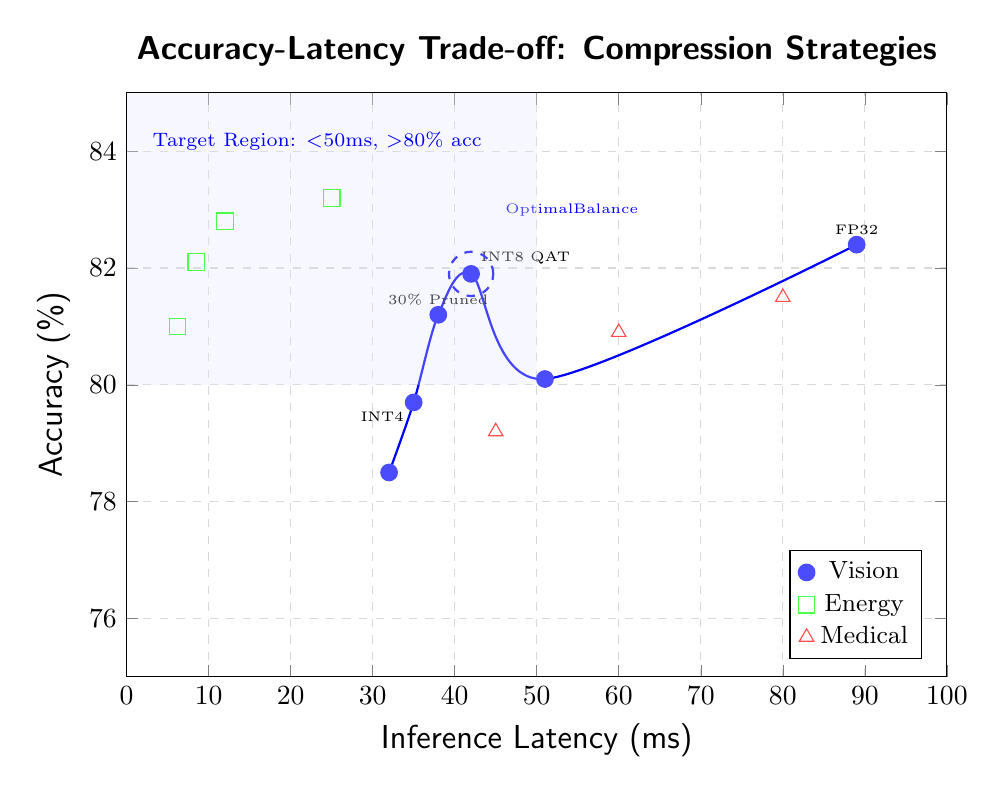
\begin{tikzpicture}
\begin{axis}[
    width=12cm,
    height=9cm,
    xlabel={Inference Latency (ms)},
    ylabel={Accuracy (\%)},
    xmin=0,
    xmax=100,
    ymin=75,
    ymax=85,
    grid=both,
    grid style={dashed, gray!30},
    legend style={at={(0.97,0.03)}, anchor=south east, font=\small},
    xlabel style={font=\large\sffamily},
    ylabel style={font=\large\sffamily},
    title={Accuracy-Latency Trade-off: Compression Strategies},
    title style={font=\large\sffamily\bfseries},
]

% Vision Jellyfish data points
\addplot[only marks, mark=*, mark size=3pt, color=blue!70]
coordinates {
    (89, 82.4)
    (42, 81.9)
    (51, 80.1)
    (35, 79.7)
    (38, 81.2)
    (32, 78.5)
};

% Energy application data
\addplot[only marks, mark=square, mark size=3pt, color=green!70]
coordinates {
    (25, 83.2)
    (12, 82.8)
    (8.5, 82.1)
    (6.2, 81.0)
};

% Medical application data
\addplot[only marks, mark=triangle, mark size=3pt, color=red!70]
coordinates {
    (80, 81.5)
    (60, 80.9)
    (45, 79.2)
};

% Draw Pareto frontier curve
\addplot[thick, blue, smooth] coordinates {
    (32, 78.5)
    (35, 79.7)
    (38, 81.2)
    (42, 81.9)
    (51, 80.1)
    (89, 82.4)
};

% Add annotations for key points
\node[font=\tiny, anchor=south west] at (axis cs:42, 81.9) {INT8 QAT};
\node[font=\tiny, anchor=south] at (axis cs:89, 82.4) {FP32};
\node[font=\tiny, anchor=north east] at (axis cs:35, 79.7) {INT4};
\node[font=\tiny, anchor=south] at (axis cs:38, 81.2) {30\% Pruned};

% Add "sweet spot" circle
\draw[blue, thick, dashed] (axis cs:42, 81.9) circle [radius=8pt];
\node[font=\tiny, text=blue, anchor=west] at (axis cs:45, 83) {Optimal\\Balance};

% Add target region
\fill[blue!10, opacity=0.3] (axis cs:0,80) rectangle (axis cs:50,85);
\node[font=\scriptsize, text=blue, anchor=north west, rotate=0] at (axis cs:2, 84.5) {Target Region: $<$50ms, $>$80\% acc};

\legend{Vision, Energy, Medical}

\end{axis}
\end{tikzpicture}
